\documentclass[12pt]{article}
\usepackage{preamble}

\pagestyle{fancy}
\fancyhead[LO,LE]{Математический анализ}
\fancyhead[CO,CE]{20.03.2024}
\fancyhead[RO,RE]{Лекции Далевской О. П.}


\begin{document}
    \hypertarget{tangentandnormaltosurface}{}

    \subsubsection{4.7.3. Касательная и нормаль к поверхности}

    Будем исследовать поверхность $\pi$ с уравнением $F(x, y, z(x, y)) = 0$ (неявное задание)

    \hypertarget{tangenttosurface}{}

    \Def Прямая $\tau$ называется касательной прямой к поверхности $\pi$ в точке $P(x, y, z)$,
    если эта прямая касается какой-либо кривой, лежащей на $\pi$ и проходящей через $P$

    \Notas Кривая получается (обычно) сечением $\pi$ какой-либо плоскостью

    \Notas В одной точке может быть множество касательных, но это не всегда так

    \Nota Договоримся различать два типа точек поверхности: обыкновенные и особые

    \Def Поверхность $\pi$ задана $F(x, y, z(x, y)) = 0$. Точка $M$ называется обыкновенной, если существуют
    все $\frac{\partial F}{\partial x}$, $\frac{\partial F}{\partial y}$, $\frac{\partial F}{\partial z}$,
    они непрерывны и не все равны нулю

    \Defs Точка $M$ называется особой, если $\frac{\partial F}{\partial x} = \frac{\partial F}{\partial y} = \frac{\partial F}{\partial z} = 0$
    или хотя бы одна из производных не существует

    \begin{MyTheorem}
        \Ths Все касательные прямые к $\pi$ в обыкновенной точке $M_0$ лежат в одной плоскости
    \end{MyTheorem}

    \begin{MyProof}
        $\vec{s}$ -- направляющий вектор касательной $\tau$, проведенной к кривой $l$ в некоторой секущей плоскости

        $d \vec{s}$ -- вектор малых приращений, то есть $d \vec{s} = (dx, dy, dz)$

        $d \vec{p}$ -- проекция $d \vec{s}$ на $Oxy$, то есть $d \vec{p} = (dx, dy)$

        Кривую $l$ можно задать параметрическими уравнениями $\begin{cases}x = \varphi(t) \\ y = \xi(t) \\ z = \theta(t)\end{cases}$

        Прямая $\tau$ имеет уравнение

        \[\frac{x - x_0}{dx} = \frac{y - y_0}{dy} = \frac{z - z_0}{dz}\]

        При отходе от $M_0$ на малое расстояние по поверхности (точнее по кривой $l$) задаем приращение $dt \neq 0$

        Домножим уравнение на $dt$

        \[\frac{x - x_0}{\frac{dx}{dt}} = \frac{y - y_0}{\frac{dy}{dt}} = \frac{z - z_0}{\frac{dz}{dt}}\]

        Из условия обыкновенности точки $M_0$ следует дифференцируемость функции $F$.
        Кроме того, уравнение можно преобразовать к виду $F(x(t), y(t), z(t)) = 0$, где $x(t), y(t), z(t)$ -- тоже дифференцируемы в точке $M_0$

        Запишем $F^\prime_t$, как вложенную:

        \[F^\prime_t = \frac{\partial F}{\partial x}\frac{dx}{dt} + \frac{\partial F}{\partial y}\frac{dy}{dt} + \frac{\partial F}{\partial z}\frac{dz}{dt} = 0\]

        Или $\left(\frac{\partial F}{\partial x}, \frac{\partial F}{\partial y}, \frac{\partial F}{\partial z}\right) \cdot \left(\frac{dx}{dt}, \frac{dy}{dt}, \frac{dz}{dt}\right) = 0$

        Таким образом, $\vec{N} \cdot \frac{d\vec{s}}{dt} = 0$. То есть $\vec{N} \perp \frac{d\vec{s}}{dt}$, при том, что $d\vec{s}$ выбран произвольно (кривая $l$ -- кривая произвольного сечения)

        Итак, вектор $\vec{N}$ перпендикулярен любой касательной $\tau$ к поверхности $\pi$ в точке $M_0$.
        Следовательно, все касательные лежат в плоскости $\kappa$ такой, что $\vec{N} \perp \kappa$
    \end{MyProof}

    \hypertarget{tangentplanetosurface}{}

    \Def Плоскость $\kappa$ (содержащая все касательные прямые $\tau$ к $\pi$ в точке $M_0$) называется касательной плоскостью к $\pi$ в $M_0$

    \Defs Прямая в направлении $\vec{N}$ через точку $M_0$ называется нормалью к $\pi$ в $M_0$

    $\vec{N}$ -- вектор нормали к поверхности в точке

    \begin{tabular}{ll}
        Уравнение ($\pi$) & $F(x, y, z) = 0, \ \vec{N} = \left(\frac{\partial F}{\partial x}, \frac{\partial F}{\partial y}, \frac{\partial F}{\partial z}\right), \ M_0(x_0, y_0, z_0) \in \pi, \kappa, n$ \\

        Касательная плоскость ($\kappa$) & $\frac{\partial F}{\partial x} (x - x_0) + \frac{\partial F}{\partial y} (y - y_0) + \frac{\partial F}{\partial z} (z - z_0) = 0$ \\

        Нормаль ($n$) & $\frac{x - x_0}{\frac{\partial F}{\partial x}} = \frac{y - y_0}{\frac{\partial F}{\partial y}} = \frac{z - z_0}{\frac{\partial F}{\partial z}}$
    \end{tabular}

    \Nota Получим вектор нормали в случае явного задания $\pi \quad z = z(x, y)$

    % https://www.geogebra.org/calculator/kd2rnuex

    \begin{wrapfigure}{R}{0pt}
        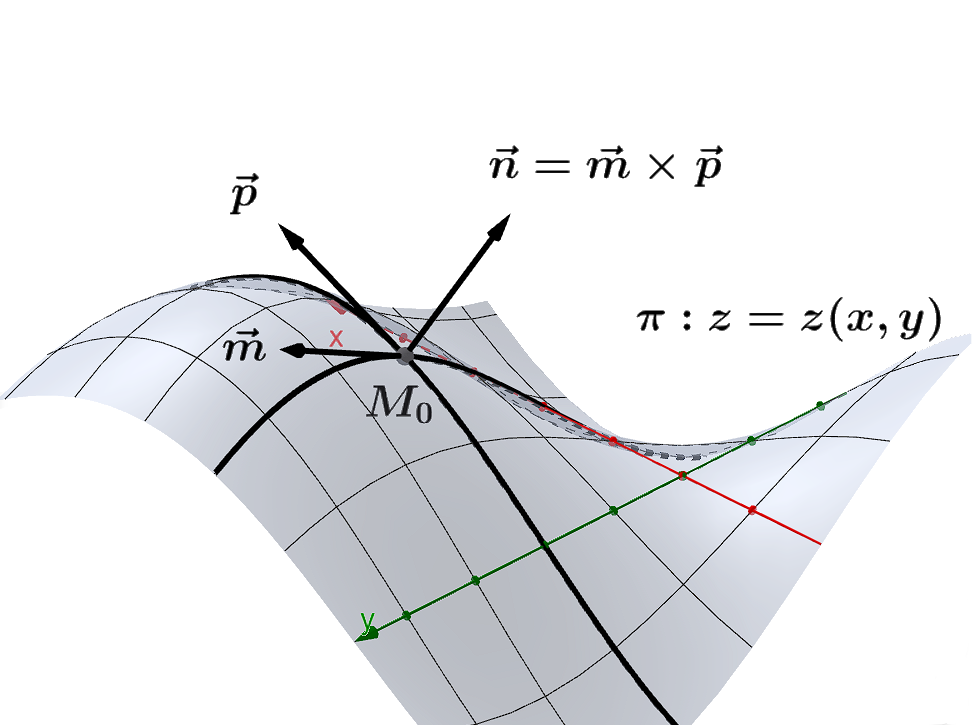
\includegraphics[width=8cm]{calculus/images/calculus_2024_03_20_1}
    \end{wrapfigure}

    Пересечем $\pi$ в точке $M_0$ плоскостями $x = x_0, y = y_0$, в сечении получим кривые с касательными векторами $\vec m$ и $\vec p$ в точке $M_0$

    Вектор нормали к $\pi$ в $M_0 \quad \vec{n} = \vec{m} \times \vec{p}$

    Найдем $\vec{m}, \vec{p}$. В сечении $x = x_0$ введем вектор $d\vec{p} || \vec{p}$:

    $d\vec{p} = \left(0, dy, \frac{\partial z}{\partial y}dy\right) = \left(0, 1, \frac{\partial z}{\partial y}\right) dy$

    Аналогично найдем $\vec{m}$ в сечении $y = y_0$:

    $\vec{m} || d\vec{m} = \left(dx, 0, \frac{\partial z}{\partial x}dx\right) = \left(1, 0, \frac{\partial z}{\partial x}\right) dx$

    Так как модуль $\vec{n}$ не важен, а только направление, то будем искать
    $\vec{n} = \left(1, 0, \frac{\partial z}{\partial x}\right) \times \left(0, 1, \frac{\partial z}{\partial y}\right)$

    \[\vec{n} =
    \begin{vmatrix} \vec\imath & \vec\jmath & \vec k \\
        1 & 0 & \frac{\partial z}{\partial x} \\ 0 & 1 & \frac{\partial z}{\partial y}
    \end{vmatrix} = \vec\imath \left(-\frac{\partial z}{\partial x}\right) - \vec\jmath \frac{\partial z}{\partial y} + \vec k = \]

    \[= \left(-\frac{\partial z}{\partial x}; -\frac{\partial z}{\partial y}; 1\right)\]

    Тогда уравнение $\kappa$:

    \[z - z_0 = \frac{\partial z}{\partial x}(x - x_0) + \frac{\partial z}{\partial y} (y - y_0) = dz\]

    Уравнение нормали $n$: $\frac{x - x_0}{-\frac{\partial z}{\partial x}} = \frac{y - y_0}{-\frac{\partial z}{\partial y}} = \frac{z - z_0}{1}$

    \Nota Последние уравнения можно получить проще, если свести уравнение $z = f(x, y)$ к уравнению $z - f(x, y) = F(x, y, z) = 0$

    \Lab Вывести уравнение $\kappa$ и $n$, пользуясь предыдущим замечанием

    \Nota Если найти $\vec{n^-} = \vec{p} \times \vec{m} = - (\vec{m} \times \vec{p})$, то получим также вектор нормали, но обращенный в противоположную сторону

    Будем говорить, что $\vec{n^+}$ - положительный вектор нормали, если угол $\angle\gamma = \angle (\vec{n^+}, Oz) \in \left[0; \frac{\pi}{2}\right)$

    $\vec{n^-}$ - отрицательный, если угол $\angle\gamma = \angle (\overrightarrow{n^-}, Oz) \in \left(\frac{\pi}{2}; \pi\right)$

    Соответственно этому верхней стороной $\pi$ называется та, у которой аппликата вектора нормали положительна

    Нижней стороне соответствует $\overrightarrow{n^-}$. Если $\overrightarrow{n} \perp Oz$, то это боковая сторона

    \subsubsection{4.7.4. Экстремумы ФНП (Ф$_2$П)}

    \hypertarget{extremumsoffunctions}{}

    \Def Точка $M_0(x_0, y_0)$ называется точкой максимума (минимума) функции $z = z(x, y)$, если $\forall M \in U_\delta (M_0) \quad z(M_0) \geq z(M)$ (для минимума $z(M_0) \leq z(M)$)

    \Nota То же, что $z(M) - z(M_0) = z - z_0 = \Delta z \leq 0$ (max), $\quad \Delta z \geq 0$ (min)

    \Mem Для функции одной переменной формулировали необходимое условие экстремума (лемма Ферма), из этого условия получали точки, подозрительные на экстремум: критические -- $f^\prime(x_0) = 0$ или $\nexists f^\prime(x_0)$ (для острого экстремума); стационарные -- $\exists f^\prime(x_0) = 0$ (частный случай критич.)

    Далее при помощи достаточных условий (признаков) проверяли наличие экстремума в критических точках

    \Nota Все термины переносятся на функции нескольких переменных. 
    Необходимое условие и достаточное условие аналогичны

    \hypertarget{extremumnecessarycondition}{}

    \begin{MyTheorem}
        \Ths Необходимое условие экстремума (гладкого):

        $z = z(x, y) : \Real^2 \rightarrow \Real$; $\quad z_0$ - точка гладкого экстремума,
        то есть $\exists \frac{\partial z}{\partial x}, \frac{\partial z}{\partial y}$ в $M_0$ и $\forall M \in U_\delta(M_0) \ z_0 \leq z(M)$ или $z_0 \geq z(M)$

        Тогда $\begin{cases}\frac{\partial z}{\partial x} \Big|_{M_0} = 0 \\ \frac{\partial z}{\partial y} \Big|_{M_0} = 0\end{cases}$
    \end{MyTheorem}

    Для существования острого экстремума нужно рассмотреть не существования или бесконечность $\frac{\partial z}{\partial x}$ или $\frac{\partial z}{\partial y}$

    Если же функция трижды дифференцируема исследования на характер экстремума можно проводить с помощью вторых производных

    \hypertarget{extremumsufficientcondition}{}

    \begin{MyTheorem}
        \Ths Достаточное условие (гладкого) экстремума

        Пусть $z = z(x, y)$ непрерывна в окрестности $M_0$ (критическая точка $\frac{\partial z}{\partial x} \Big|_{M_0} = 0, \frac{\partial z}{\partial y} \Big|_{M_0} = 0$)
        вместе со своими первыми и вторыми производными (можно потребовать трижды дифференцируемость)

        Тогда, если $\frac{\partial^2 z}{\partial x^2} \stackrel{\text{обозн}}{=} A, \frac{\partial^2 z}{\partial x \partial y} \stackrel{\text{обозн}}{=} B, \frac{\partial^2 z}{\partial y^2} \stackrel{\text{обозн}}{=} C$, то

        \begin{enumerate}
            \item $AC - B^2 > 0, A > 0 \Longrightarrow M_0$ -- точка минимума
            \item $AC - B^2 > 0, A < 0 \Longrightarrow M_0$ -- точка максимума
            \item $AC - B^2 < 0 \Longrightarrow$ в точке $M_0$ нет экстремума
            \item $AC - B^2 = 0\Longrightarrow$ нельзя утверждать наличие или отсутствие экстремума в точке (требуются дополнительные исследования)
        \end{enumerate}
    \end{MyTheorem}

    $\Box$

    Функция $z$ дважды дифференцируема, тогда ($z_0 = z(M_0)$)

    $\Delta z = z - z_0 = \frac{dz}{1!} |_{M_0} + \frac{d^2 z}{2!} |_{M_0} + o((\Delta \rho)^2) \quad \Delta \rho = \sqrt{(\Delta x)^2 + (\Delta y)^2} = \sqrt{(dx)^2 + (dy)^2}, \ dx = \Delta\rho \cos\alpha, dy = \Delta\rho \sin\alpha$

    $o((\Delta \rho)^2) = \lambda (\Delta \rho)^3$

    Заметим, что $dz |_{M_0} = 0$, так как $M_0$ - критическая

    $d^2 z = \left(\frac{\partial}{\partial x} + \frac{\partial}{\partial y}\right)^2 z = \left(\frac{\partial^2}{\partial x^2} + 2 \frac{\partial^2}{\partial x \partial y} + \frac{\partial^2}{\partial y^2}\right) z =
    \frac{\partial^2 z}{\partial x^2} (dx)^2 + 2 \frac{\partial^2 z}{\partial x \partial y} dxdy + \frac{\partial^2 z}{\partial y^2} (dy)^2 = A (dx)^2 + 2B dxdy + C(dy)^2 =
    A(\Delta \rho)^2 \cos^2\alpha + 2B (\Delta \rho)^2 \cos\alpha\sin\alpha + C(\Delta \rho)^2 \sin^2\alpha$

    Тогда $\Delta z = \frac{1}{2} (\Delta \rho)^2 (A\cos^2\alpha + 2B\cos\alpha\sin\alpha + C\sin^2\alpha + 2\lambda \Delta \rho)$

    Далее рассмотрим отдельно случаи $A \neq 0$ и $A = 0$

    $A \neq 0$: $A\cos^2\alpha + 2B\cos\alpha\sin\alpha + C\sin^2\alpha = \frac{A^2\cos^2\alpha + 2AB\cos\alpha\sin\alpha + B^2\sin^2\alpha + (AC - B^2)\sin^2\alpha}{A} =
    \frac{(A\cos\alpha + B\sin\alpha)^2 + (AC - B^2)\sin^2\alpha}{A}$

    1) $\sqsupset AC - B^2 > 0 (A > 0)$: Числитель неотрицательный и не равен нулю (иначе $\sin\alpha = 0$, то тогда $A\cos\alpha \neq 0$)

    Итак, числитель и знаменатель больше нуля. Обозначим всю дробь за $k^2 > 0$

    Вернемся к $\Delta z = \frac{1}{2}(\Delta \rho)^2 (k^2 + 2\lambda\Delta\rho)$

    Устремим $\Delta \rho \rightarrow 0$, начиная с какого-то $\delta \ \forall M \in U_\delta(M_0) \ k^2 + \lambda\Delta\rho > 0$

    То есть $\Delta z > 0$ в $U_\delta(M_0) \Longrightarrow M_0$ - точка минимума (локально в $U_\delta(M_0)$)

    2) $\sqsupset AC - B^2 > 0 (A < 0)$, тогда $\Delta z = \frac{1}{2}(\Delta \rho)^2 (-k^2 + 2\lambda\Delta\rho) < 0$ при достаточно малом $\Delta \rho$

    3) $\sqsupset AC - B^2 < 0 (A > 0)$, тогда фиксируем направления $\alpha = 0 \Longrightarrow \sin\alpha = 0$

    $\Delta z = \frac{1}{2}(\Delta \rho)^2 (A + 2\lambda\Delta\rho) > 0$

    $tg \alpha = -\frac{A}{B} \Longrightarrow \frac{(AC - B^2)\sin^2\alpha}{A} = -k^2, \Delta z = \frac{(\Delta \rho)^2}{2}(-k^2 + 2\lambda\Delta\rho) < 0$

    Вдоль разных путей $\alpha = 0$, $tg \alpha = -\frac{A}{B}$, разный знак $\Delta z \Longrightarrow$ нет экстремума

    \Nota Можно аналогично рассмотреть $A < 0$

    4) $A = 0$, вернемся к выражению $\Delta z = \frac{1}{2} (\Delta \rho)^2 (\sin\alpha(2B\cos\alpha + C\sin\alpha) + 2\lambda\Delta\rho)$

    Пусть $\alpha$ беск. мал, тогда $\sin\alpha \approx 0, C\sin\alpha \approx 0, 2B\cos\alpha \approx 2B$. Тогда знак $\sin\alpha \cdot 2B$ зависит от $\alpha$

    То есть $\Delta z$ колеблется вместе с $\alpha$ по знаку $\Longrightarrow$ нет экстремума

    Можно доказать при $A \neq 0$, например, выбрав $tg \alpha = -\frac{A}{B}$, что знак $\Delta z$ зависит от $\alpha$

    $\Box$

\end{document}
